\section{The Goal Structuring Notation}
\label{gsn}
It is necessary to discuss the Goal Structuring Notation (GSN) before discussing SACM as SACM was developed based on the concepts in GSN. GSN is a well established graphical argumentation notation to represent safety arguments in a structured way. GSN captures elements that form safety argument, and the relationships between the elements. GSN is widely adopted within safety-critical industries for the presentation of safety arguments within safety cases. The core elements of GSN is shown in Figure~\ref{fig:gsnCore}.

\begin{figure}
	\centering
	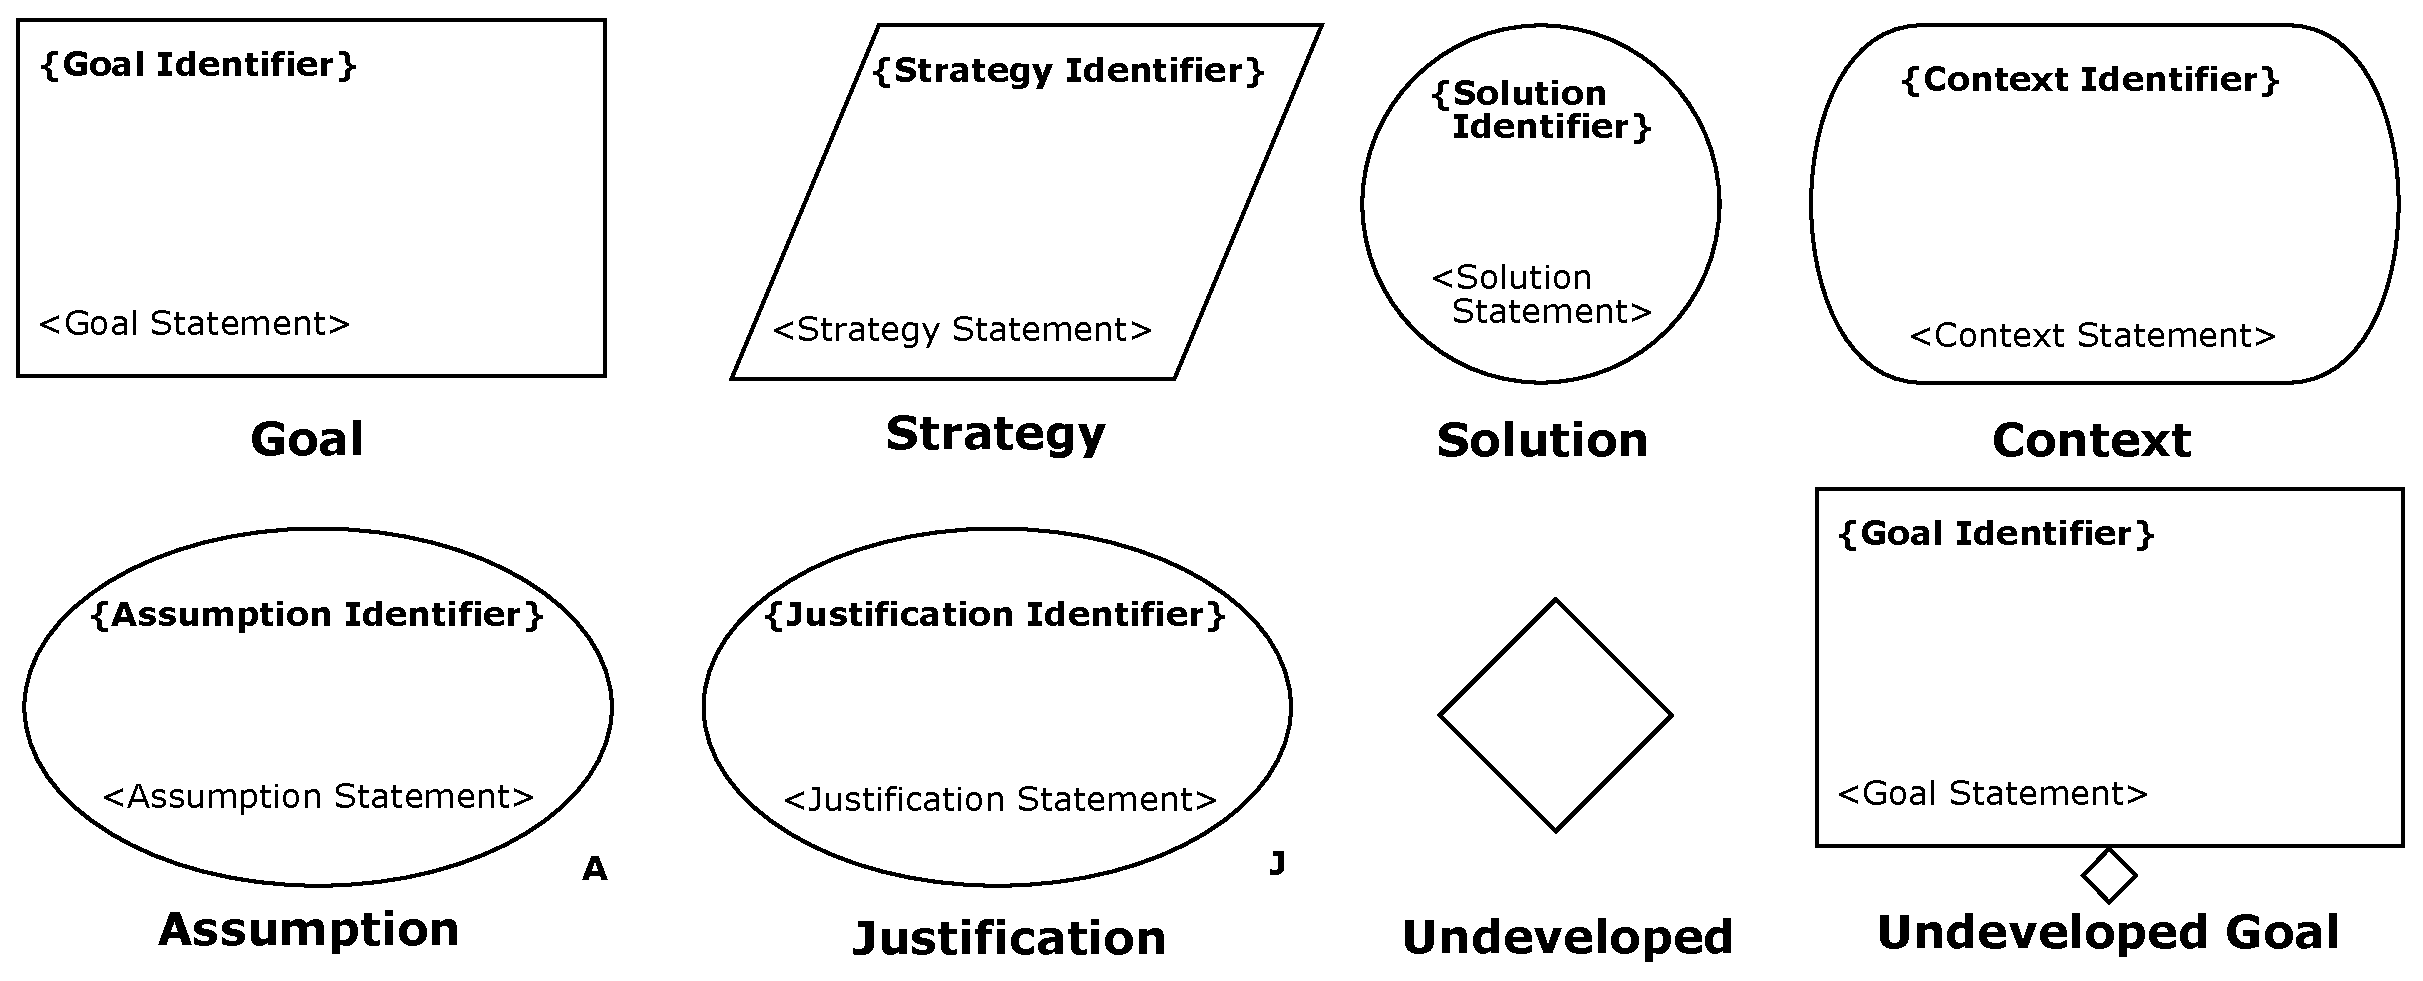
\includegraphics[width=1\linewidth]{basicGSN.eps}
	\caption{Core GSN Elements}
	\label{fig:gsnCore}
\end{figure}

A \textit{Goal} represents a claim within the argumentation. A \textit{Strategy} is used to describe the nature of the inference that exists between a goal and its supporting goal(s). A \textit{Solution} represents a reference to an evidence item or multiple evidence items. A \textit{Context} represents a contextual artefact, which can be a statement, or a reference to contextual information. An \textit{Assumption} represents an assumed statement made within the argumentation. A \textit{Justification} represents a statement of rationale. An element can be \textit{Undeveloped}, which means that a line of argument has not been developed yet, it can apply to \textit{Goal}s and \textit{Strategies}, the \textit{Undeveloped Goal} in Figure~\ref{fig:gsnCore} provides an example. 

\begin{figure}
	\centering
	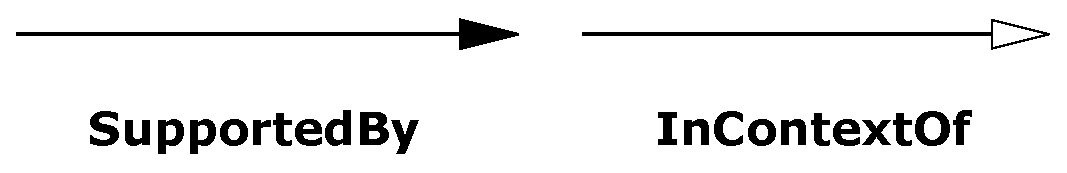
\includegraphics[width=0.5\linewidth]{gsnConnectors.eps}
	\caption{Core GSN Elements}
	\label{fig:gsnEdges}
\end{figure}

Core elements of GSN are connected with two types of edges, as shown in Figure~\ref{fig:gsnEdges}. The \textit{SupportedBy} edge allows inferential or evidential relationships to be documented. The \textit{InContextOf} relates contextual elements (i.e. \textit{Context}, \textit{Assumption} and \textit{Justification}) to \textit{Goal}s and \textit{Strategies}.

When the elements of the GSN are linked together in a network, they are described as a \textit{goal structure}. The purpose of any goal structure is to show how \textit{Goal}s are successively broken down into sub-\textit{Goal}s until a point is reached where claims can be supported by direct reference to available evidence (\textit{Solution}s). An example goal structure is shown in Figure~\ref{fig:goalStructure}.

\begin{figure}
	\centering
	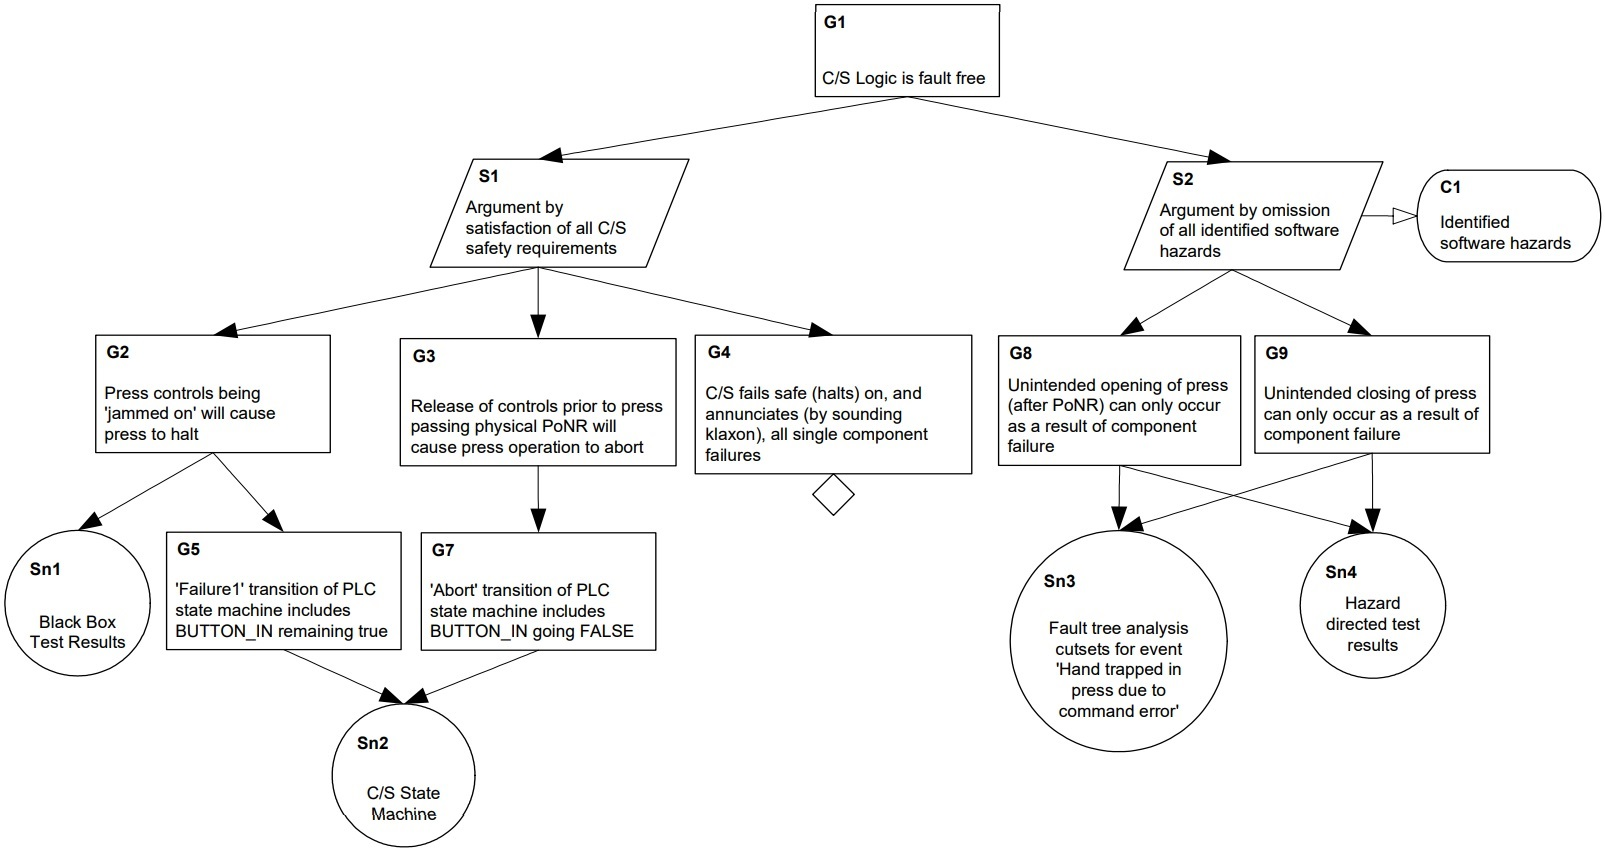
\includegraphics[width=1\linewidth]{GSNExample.jpg}
	\caption{An example goal structure}
	\label{fig:goalStructure}
\end{figure}
Figure~\ref{fig:modularGSN} shows how GSN supports modularity. Goal structures can be organised in \textit{Module}s. For example, for a system that consists two components A and B, it is possible to organise the safety case of component A in Module A and safety case of component B in Module B. Modularity promotes re-use, so that safety cases for system components can be re-used when different components integrate to form a system. When integrating system safety case, a \textit{Contract Module} can be used to \textit{bind} different \textit{Module}s together. Binding is done via the use of \textit{Away Goal}s, \textit{Away Context}s and \textit{Away Solution}, where \textit{Goal}s, \textit{Context}s and \textit{Solution}s from an external \textit{Module} can be referenced. Like other GSN elements, away elements can be connected using \textit{SupportedBy} and \textit{InContextOf} edges.

\begin{figure}
	\centering
	\includegraphics[width=0.9\linewidth]{ModularGSN.eps}
	\caption{Modular GSN Elements}
	\label{fig:modularGSN}
\end{figure}

GSN also provides the extension for users to define \textit{GSN Pattern}s to re-use good practice of safety cases. In \cite{kelly1997safety}, the use of patterns are discussed, patterns are a means of documenting and reusing successful assurance argument structures. Safety case argument patterns provide a way of capturing the required form of a safety argument in a manner that is abstract from the details of a particular argument. It is then possible to use the patterns to create specific arguments by \textit{instantiating} the patterns in a manner appropriate to the application. Pattern instantiation refers to the process of constructing concrete system safety cases by filling in the templates provided in the GSN pattern with actual system information. Figure~\ref{fig:gsnPatterns} shows the elements in GSN which enables the users to create patterns.

\begin{figure}
	\centering
	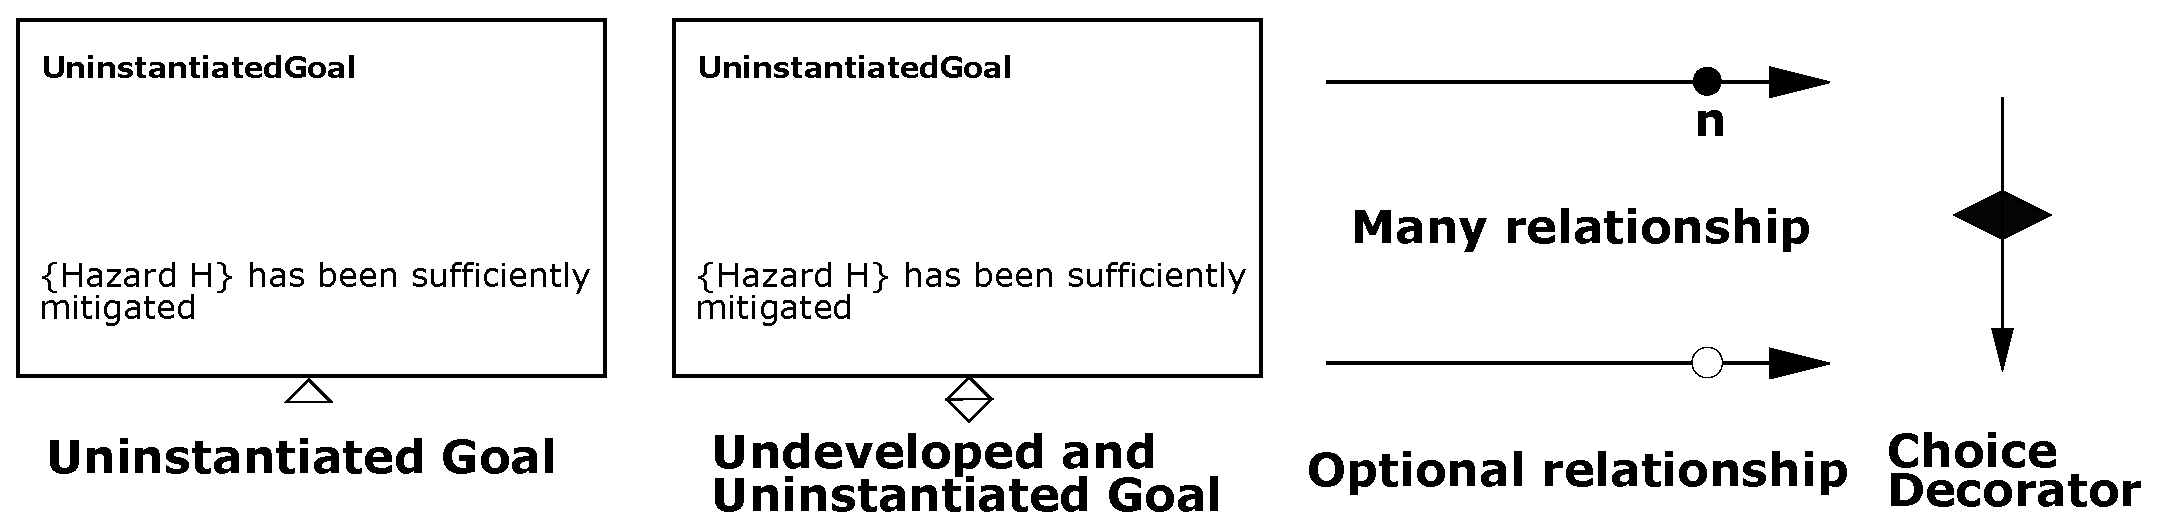
\includegraphics[width=1\linewidth]{gsnPattern.eps}
	\caption{An example goal structure}
	\label{fig:gsnPatterns}
\end{figure}

The \textit{Uninstantiated} indicator marks that an element is abstract and to be instantiated, at some later stage, the abstract element needs to be replaced with a more concrete instance. \textit{Uninstantiated indicator} can be associated to any GSN element, Figure~\ref{fig:gsnPatterns} demonstrates how it can be associated to an \textit{Goal}. The \textit{Undeveloped and Uninstantiated} indicator marks an element (in particular, \textit{Goal}s and \textit{Strategies}) is both abstract (to be instantiated) and needs more development (needs supporting argument), Figure~\ref{fig:gsnPatterns} demonstrates its usage on a Goal. In GSN patterns, the \textit{SupportedBy} and \textit{InContextOf} connector can bear more information, the \textit{Many} decorator on a connector indicates that when the pattern is instantiated, the connector can be multiplied \textit{n} times (expressed in the label) based on the actual system information provided. The \textit{Optional} decorator indicates that when the pattern is instantiated, the connector can connect to one or zero element. The \textit{Choice} decorator on a connector can be used to denote possible alternatives in satisfying a relationship. It can represent 1-of-n and m-of-n selection. 

\begin{figure}[ht!]
	\centering
	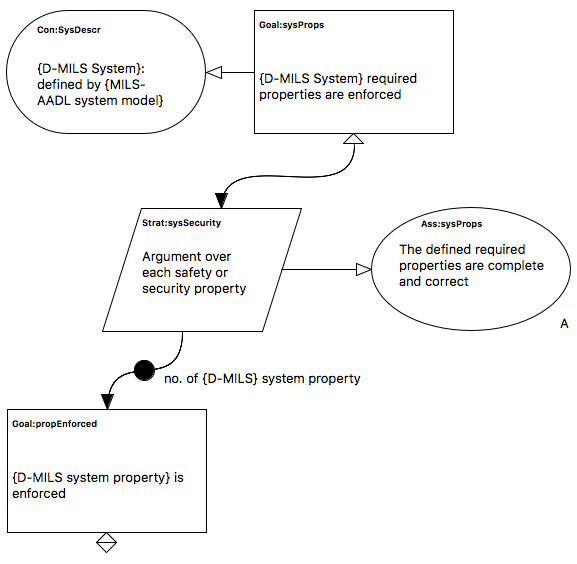
\includegraphics[width=.8\linewidth]{D-MILS-example.png}
	\caption{An example of GSN Pattern for the D-MILS Project \cite{}}
	\label{fig:dmilsPattern}
\end{figure}

Figure~\ref{fig:dmilsPattern} shows an example of GSN pattern (partially shown due to space limit). The contents in the curly brackets are \textit{role}s in GSN terms, they are place holders which when the pattern is instantiated, will be replaced by actual system information (in this case, Distributed Multiple Independent Levels of Security - D-MILS systems). The \{D-MILS System\} in \textit{Goal:sysProps} will be replaced with the actual name of the D-MILS system when the pattern is instantiated. Similarly, the \textit{SupportedBy} connector between \textit{Strat:sysSecurity} and \textit{Goal:propEnforced} specifies that when the pattern is instantiated, there should be $N$ (the number of D-MILS system property) \textit{Goal}s and $N$ \textit{SupportedBy} connected to \textit{Strat:sysSecurity}. Pattern instantiation if often an manual process that involves comprehension of the GSN patterns and replacing the \textit{role}s with actual system information. However, there has been work on automating the pattern instantiation process using MDE with the use of a \textit{weaving model} \cite{hawkins2015weaving}. 

In this section, we discussed briefly the elements provided by GSN. GSN is powerful in representing arguments in a structured way, which enables better comprehension of system safety arguments. GSN promotes modularity and abstraction in the sense that good practice in safety case construction can be captured and re-used. In the following sections, we will discuss SACM and its relationship with GSN. 